\section*{Neuromatch}%
\sectionauthor{Enabling inclusinve collaborative and global participation in the computational sciences}

\begin{figure}[!h]
  \centering
  
\includegraphics[width=0.8\textwidth]{images/neuromatch-logo-2-transparent}
\end{figure}

Neuromatch is a nonprofit organization (registered as a 501(c)(3) in the U.S.) training the next generation of global computational research leaders.

\section*{Neuromatch Academy}
\sectionauthor{\vspace{-4ex}}

Applications for our Neuromatch Academy open 16 February until 15 March.
Neuromatch run virtual courses in Computational Neuroscience, NeuroAI, Deep Learning, and Computational Tools for Climate Science in July.
More information at: \href{https://neuromatch.io/courses/}{https://neuromatch.io/courses/}.
\vspace{1ex}

\begin{figure}[!h]
  \centering
  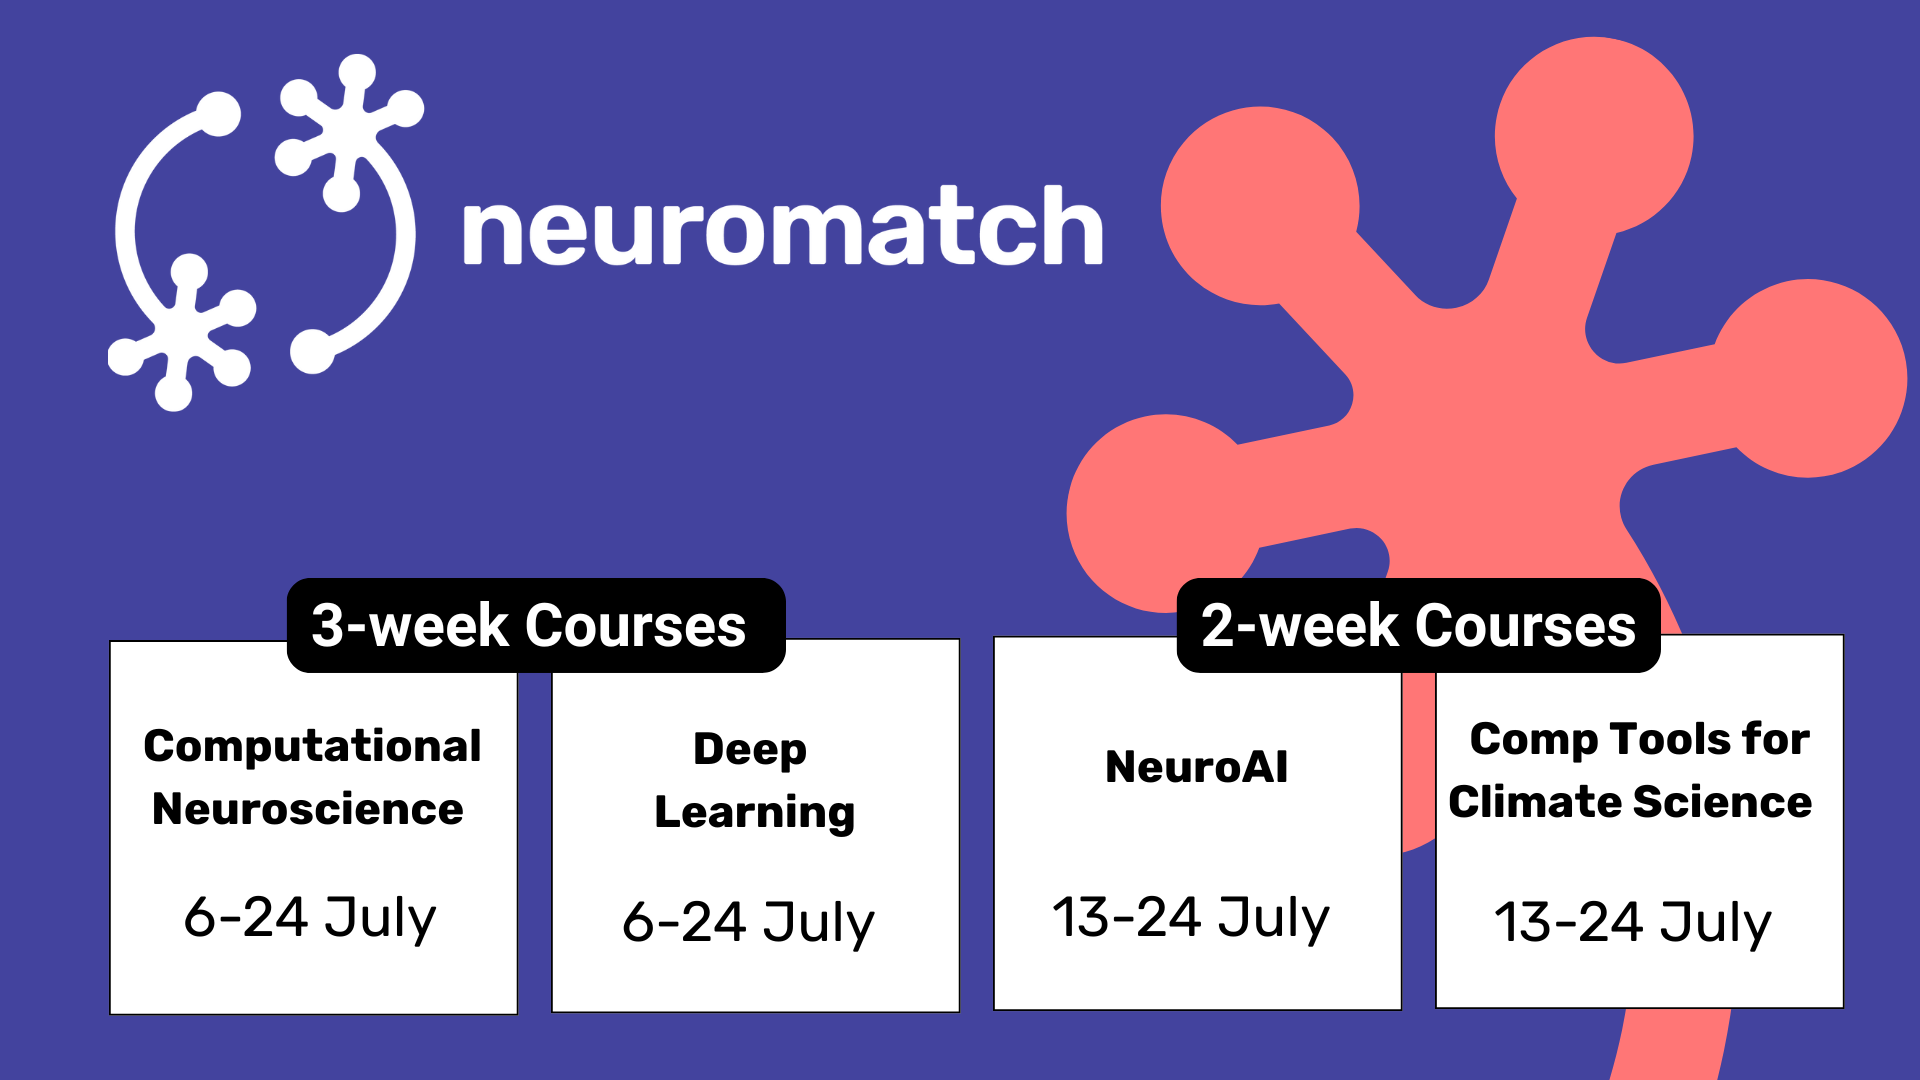
\includegraphics[width=0.8\textwidth]{images/2026-nma}
\end{figure}

\section*{Connect with Neuromatch}
\sectionauthor{\vspace{-4ex}}
\vspace{1ex}
\begin{center}
  \href{https://twitter.com/neuromatch?lang=en}{\vcenteredinclude{./images/X-logo}}~
  \href{https://www.facebook.com/Neuromatch/}{\vcenteredinclude{./images/Facebook_icon_2013.svg}}~
  \href{https://neuromatch.social/@neuromatch}{\vcenteredinclude{./images/mastodon}}~
  \href{https://www.linkedin.com/company/neuromatch}{\vcenteredinclude{./images/LinkendIn}}~
  \textbf{\Large @Neuromatch}
\end{center}
\vspace{1ex}
